%\documentclass[fleqn]{book}
\documentclass[11pt]{amsbook}

\usepackage[turkish]{babel}

%\usepackage{../HBSuerDemir}	% ------------------------
\usepackage{../Ceyhun}	% ------------------------
\usepackage{../amsTurkish}


\begin{document}
% ++++++++++++++++++++++++++++++++++++++
\hPage{44}
\begin{figure}[htb]
	\centering
	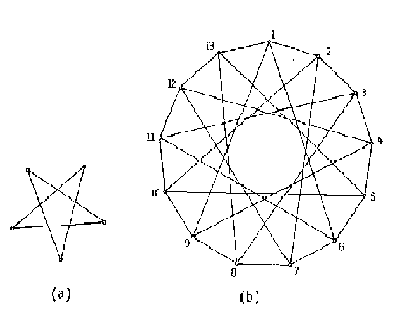
\includegraphics[width=0.45\textwidth]{images/ceyhun-044-fig01}
	\caption{R(3,3)=6 ve R(3,5)=14 olduğunu gösteren çizgeler}
\end{figure}
\par Benzer olarak, $m=3$ ve $n=5$ için, Teorem 1.6.1
$$ R(3,5) \leq \binom{6}{2} = \frac{6!}{2!4!} = 15$$ 
Teorem 1.6.2 ise,
$$R(3,5) \leq \frac{28}{2} = 14$$
verecektir. Demek ki $R(3,5) \leq 14$ tür. Ancak ,
% ++++++++++++++++++++++++++++++++++++++


\end{document}